\subsection{Problem 2.4:}
\begin{enumerate}
    \item Chứng minh mọi tín hiệu đều phân tích được thành tổng của một thành phần chẵn và một thành phần lẻ:\\
    Ta có đồng nhất thức:
    \[
    x(n) = \frac{1}{2}[x(n) + x(-n)] + \frac{1}{2}[x(n) - x(-n)]
    \]
    Đặt:
    \[
    \begin{cases}
        x_e(n) = \frac{1}{2}[x(n) + x(-n)] \\
        x_o(n) = \frac{1}{2}[x(n) - x(-n)]
    \end{cases}
    \]
    Ta kiểm tra:
    \begin{itemize}
        \item Tính chẵn của $x_e(n)$:
        $$
        x_e(-n) = \frac{1}{2}[x(-n) + x(n)] = x_e(n) \rightarrow x_e(n) \text{ là tín hiệu chẵn}
        $$
        \item Tính lẻ của $x_o(n)$:
        $$
        x_o(-n) = \frac{1}{2}[x(-n) - x(n)] = -\frac{1}{2}[x(n) - x(-n)] = -x_o(n) \rightarrow x_o(n) \text{ là tín hiệu lẻ}
        $$
    \end{itemize}
    Ta có: $x_e(n) + x_o(n) = x(n)$.\\
    \textbf{Kết luận:} Mọi tín hiệu đều phân tích được thành tổng một thành phần chẵn và một thành phần lẻ.

    \item Sự phân tích trên có phải là duy nhất không (Tính duy nhất)?\\
    Giả sử tồn tại một phân tích khác: $x(n) = x'_e(n) + x'_o(n)$ với $x'_e(n)$ là tín hiệu chẵn, $x'_o(n)$ là tín hiệu lẻ.\\
    Khi đó xét tín hiệu đảo:
    $$
    x(-n) = x'_e(-n) + x'_o(-n) = x'_e(n) - x'_o(n)
    $$
    Ta có hệ phương trình:
    \[
    \begin{cases}
        x(n) = x'_e(n) + x'_o(n) \\
        x(-n) = x'_e(n) - x'_o(n)
    \end{cases}
    \rightarrow
    \begin{cases}
        x'_e(n) = \frac{1}{2}[x(n) + x(-n)] = x_e(n) \\
        x'_o(n) = \frac{1}{2}[x(n) - x(-n)] = x_o(n)
    \end{cases}
    \]
    \textbf{Kết luận:} Sự phân tích thành phần chẵn và lẻ là duy nhất.

    \item Minh họa với tín hiệu $x(n) = \{2, 3, \underset{\uparrow}{4}, 5, 6\}$ ($n \in [-2, 2]$):\\
    Ta có:
    \[
    \begin{cases}
        x(n) = \{2, 3, \underset{\uparrow}{4}, 5, 6\} \\
        x(-n) = \{6, 5, \underset{\uparrow}{4}, 3, 2\}
    \end{cases}
    \]
    - Thành phần chẵn $x_e(n) = \frac{x(n) + x(-n)}{2}$:
    \[
    \begin{cases}
        x_e(-2) = \frac{2 + 6}{2} = 4 \\
        x_e(-1) = \frac{3 + 5}{2} = 4 \\
        x_e(0)  = \frac{4 + 4}{2} = 4 \\
        x_e(1)  = \frac{5 + 3}{2} = 4 \\
        x_e(2)  = \frac{6 + 2}{2} = 4
    \end{cases}
    \rightarrow x_e(n) = \{4, 4, \underset{\uparrow}{4}, 4, 4\}
    \]
    - Thành phần lẻ $x_o(n) = \frac{x(n) - x(-n)}{2}$:
    \[
    \begin{cases}
        x_o(-2) = \frac{2 - 6}{2} = -2 \\
        x_o(-1) = \frac{3 - 5}{2} = -1 \\
        x_o(0)  = \frac{4 - 4}{2} = 0 \\
        x_o(1)  = \frac{5 - 3}{2} = 1 \\
        x_o(2)  = \frac{6 - 2}{2} = 2
    \end{cases}
    \rightarrow x_o(n) = \{-2, -1, \underset{\uparrow}{0}, 1, 2\}
    \]
    Kiểm tra lại: $x_e(n) + x_o(n) = \{4 - 2, 4 - 1, 4 + 0, 4 + 1, 4 + 2\} = \{2, 3, \underset{\uparrow}{4}, 5, 6\} = x(n)$.
\end{enumerate}

\begin{figure}[H]
    \centering
    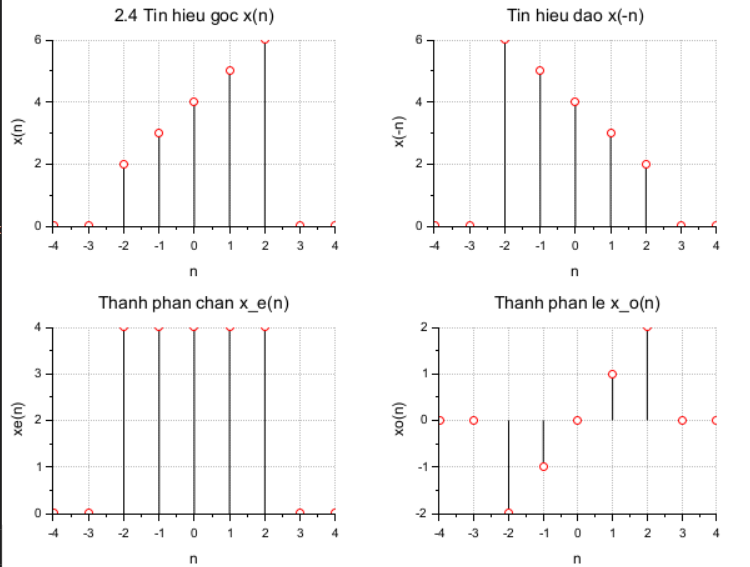
\includegraphics[width=0.75\textwidth]{img/ad_ex2.4.png}
    \caption{Đồ thị mô phỏng kết quả Problem 2.4 trên Scilab}
\end{figure}
